\documentclass[a4paper,12pt]{report}
\usepackage{url}
\usepackage{enumitem}
\usepackage{palatino}
\usepackage[cmex10]{amsmath}
\usepackage{stmaryrd,amssymb}
\usepackage{graphicx}
\usepackage{amsfonts}
\usepackage{rotating}
\usepackage{listings}
\usepackage{xcolor}
\usepackage{url,boxedminipage,listings}
\usepackage{booktabs}
\usepackage{rotating}
\usepackage{array}
\usepackage{color,url,varioref,xcolor}
\usepackage{alltt,epsfig,comment}
\usepackage{supertabular,fancyhdr}
\usepackage{multirow}
\usepackage{url}
\usepackage{xspace}
\usepackage{dsfont}
\usepackage[english]{babel}
\usepackage{todonotes}

\usepackage{pdfpages}
\usepackage[font={footnotesize,sl}, labelfont=bf] {caption}

\usepackage{tikz}
\usetikzlibrary{arrows}
\usetikzlibrary{automata}
\usetikzlibrary{positioning}
\usetikzlibrary{er}

% HAS TO BE LAST PACKAGE:
\usepackage[pdftex,bookmarks=true,pageanchor=false]{hyperref}



% Eiffel Code Stuff
\lstset{language=OOSC2Eiffel,basicstyle=\ttfamily\small}
\definecolor{codebg}{rgb}{0.95,0.95,0.95}
\setlength{\headheight}{28pt}

% Inline Eiffel Code
\let\e\lstinline
% Eiffel Identifiers or expressions
\newcommand{\eid}[1]{\textsl{{\color[HTML]{000000} #1}}}
% Eiffel Class names
%\newcommand{\ecl}[1]{\textsl{{\color[HTML]{3333FF} #1}}}
\newcommand{\ecl}[1]{\textsl{{\color[HTML]{000000} #1}}}
% Eiffel Keywords
%\newcommand{\ekey}[1]{\textbf{{\color[HTML]{333399} #1}}}
\newcommand{\ekey}[1]{\textbf{{\color[HTML]{000000} #1}}}

\newcommand{\distance}[2]{\ensuremath{#1\leftrightarrow#2}}

\lstset{escapechar=\$}

\newcommand{\blankpage}{
\newpage
\thispagestyle{empty}
\mbox{}
\newpage
}


\title {The ABEL Persistence Library Tutorial}
\author {
	Roman Schmocker, Marco Piccioni\\\\
	Last updated:
}


\begin{document}

%\pagenumbering{roman}
%
\includepdf {includes/title_page}
\maketitle

%\blankpage

%\section*{Abstract}

ABEL is an approach to wrap every existing persistence library under a simple and yet powerful API.
The programming interface of ABEL is completely transparent to the actual storage mechanism, and it supports the CRUD operations, transactions, and some advanced features like result filtering based on some criteria.

ABEL has a flexible framework that allows to adapt the API to basically any existing persistence solution.
The framework has a reusable object-relational mapper at its core and is open for extensions and customization.

%\blankpage

\tableofcontents

%\chapter{Introduction}
\pagenumbering{arabic}


%\section{Introduction}

The Eiffel language \cite{EcmaEiffel} \cite{Meyer09} has a lot of different persistence libraries, and every solution has its own advantages and drawbacks.
A database such as MySQL \cite {MySQL} for example is quite fast, but it comes at the expense of the object-relational impedance mismatch \cite{ORImpedance}.
A serialization library on the other hand is easier to handle for the programmer, but its performance rapidly decreases for large data sets.

It is very hard to switch from one persistence solution to another, because all have their own interface.
Even changing for example the data\-base from MySQL to Oracle \cite{Oracle} is usually very hard to achieve, if only because their SQL dialects are different.

To overcome such problems we have developed a new library called ABEL, which is the acronym for ``A better Eiffelstore library''.
ABEL tries to unify existing persistence libraries unter a simple and yet powerful API, which is completely transparent to the actual storage mechanism.


\section{Overview}
This thesis is basically splitted into two parts: The API tutorial and the technical documentation.

In the first part you will be introduced to the basic operations of the API, like the CRUD (Create, Read, Update, Delete) operations or transaction handling.

The second part is an introduction to the general architecture of ABEL and some selected topics like the object-relational mapping layer or the main interfaces for backend abstraction.

\chapter{Introducing ABEL}
ABEL (A Better EiffelStore Library) is an object-oriented persistence library written in Eiffel and aiming at seamlessly integrating various kinds of data stores.
 
\section{Setting things up}
We are assuming you have checked out the ABEL code from the EiffelStudio SVN repository\footnote{https://svn.eiffel.com/eiffelstudio/branches/eth/eve/Src/library/abel}, and have EiffelStudio installed. Launch it and in the initial window choose "tutorial\_project". If it is not there just push "Add project" and navigate to the location where you downloaded ABEL, and look for the \emph{tutorial\_project.ecf} project file in \emph{abel/apps/sample/tutorial/}. You can then load and compile the project. To be able to compile the ABEL tutorial you don't need particular dependencies, because we are using an in-memory database simulating a relational database. If you want to experiment with ABEL's support for a full-fledged relational back-end (like MySQL or SQLite, see Chapter~\ref{chapter:advanced_initialization}), you need to install the databases and the appropriate drivers.

\section{Getting started}
We will be using \lstinline!PERSON! objects to show the usage of the API. 
In the source code below you will see that ABEL handles objects "as they are", meaning that to make them persistent you don't need to add any dependencies to their class source code.

\begin{lstlisting}[language=OOSC2Eiffel, captionpos=b, caption={The PERSON class}, label={lst:person_class}]
class PERSON

create
	make

feature {NONE} -- Initialization

	make (first, last: STRING)
			-- Create a newborn person.
		require
			first_exists: not first.is_empty
			last_exists: not last.is_empty
		do
			first_name := first
			last_name := last
			age:= 0
		ensure
			first_name_set: first_name = first
			last_name_set: last_name = last
			default_age: age = 0
		end

feature -- Basic operations

	celebrate_birthday
			-- Increase age by 1.
		do
			age:= age + 1
		ensure
			age_incremented_by_one: age = old age + 1
		end

feature -- Access

	first_name: STRING
		-- The person's first name.

	last_name: STRING
		-- The person's last name.

	age: INTEGER
		-- The person's age.

invariant
	age_non_negative: age >= 0
	first_name_exists: not first_name.is_empty
	last_name_exists: not last_name.is_empty
end

\end{lstlisting}

There are three very important classes in ABEL:
\begin{itemize}
 \item The deferred class \lstinline!PS_REPOSITORY! provides an abstraction to the actual storage mechanism.
 \item The \lstinline!PS_CRUD_EXECUTOR! class is, as the name suggests, responsible to execute CRUD (Create Read Update Delete) commands. Every \lstinline!PS_CRUD_EXECUTOR! object works with a \lstinline!PS_REPOSITORY!.

 \item The \lstinline!PS_OBJECT_QUERY [G]! class is used to describe a read operation over objects of type \lstinline!G!. You can execute such a query in the \lstinline!PS_CRUD_EXECUTOR!. 
	The result will be objects of type \lstinline!G!.

 
\end{itemize}
To start using the library, we first need to create an object of type\\
\lstinline!PS_REPOSITORY!. In this case we will be creating a more specific object of type \lstinline!PS_IN_MEMORY_REPOSITORY!. \\
As a second step, we need to create an object of type  \lstinline{PS_CRUD_EXECUTOR}, useful to execute CRUD operations. To create it, we will pass as an argument to its creation feature the previously created repository.

\begin{lstlisting}[language=OOSC2Eiffel, captionpos=b, caption={The TUTORIAL class}, label={lst:tutorial_class}]
class TUTORIAL

create
	make

feature {NONE} -- Initialization

	make
		-- Set up a simple in-memory repository.
		local
			repository: PS_IN_MEMORY_REPOSITORY
		do
			create repository.make_empty
			create executor.make (repository)
		end

feature
	
	executor: PS_CRUD_EXECUTOR
		-- The CRUD executor used throughout the tutorial.

end
\end{lstlisting}
We will use this class throughout the tutorial. You can assume that the Eiffel features listed in this tutorial are located inside the \lstinline!TUTORIAL! class, if they are not enclosed in another class declaration.\\ 
We encourage you to test the features shown in this tutorial by calling them from feature \lstinline{explore} in class \lstinline!TUTORIAL!.
\chapter{Basic operations}

\section{Inserting}

You insert an object in the repository using feature \lstinline{insert} in class\\ 
\lstinline{PS_CRUD_EXECUTOR}. Let's add three new persons to the database in feature \lstinline{explore}:
\begin{lstlisting}[language=OOSC2Eiffel, captionpos=b, caption={Insertion code.}, label={lst:tutorial_insert}]
	explore
			-- Tutorial code.
		local
			p1, p2, p3: PERSON
		do
			-- Insert 3 new persons in the database
			create p1.make ("Albo", "Bitossi")
			p1.celebrate_birthday
			executor.insert (p1)
			create p2.make ("Berno", "Citrini")
			p2.celebrate_birthday
			p2.celebrate_birthday
			p2.celebrate_birthday
			executor.insert (p2)
			create p3.make ("Dumbo", "Ermini")
			executor.insert (p3)			
		end
\end{lstlisting}

\section{Querying}
\label{section:querying}
A query for objects is done by creating a \lstinline!PS_OBJECT_QUERY [G]! object and executing it using features of \lstinline!PS_CRUD_EXECUTOR!.
The generic parameter \lstinline!G! denotes the type of objects that should be queried.

After a successful execution of the query, you can find the result in the iteration cursor \lstinline{result_cursor} in class \lstinline{PS_OBJECT_QUERY}. The feature \lstinline{simple_query} below shows how to get a list of persons from the repository:
%Having an iteration cursor as a result has several advantages, e.g. support for lazy loading or the across syntax, as you will see in the next example:

\begin{lstlisting}[language=OOSC2Eiffel, captionpos=b, caption={A simple query.}, label={lst:simple_query}]
	simple_query: LINKED_LIST [PERSON]
		-- Query all persons from the current repository.
		local
			query: PS_OBJECT_QUERY [PERSON]
		do
			create Result.make
			create query.make
			executor.execute_query (query)

			across query as	query_result
			loop
				Result.extend (query_result.item)
			end
		end
\end{lstlisting}
We now add in feature \lstinline{explore} the code to print the linked list returned by feature \lstinline{simple_query}:  
\begin{lstlisting}[language=OOSC2Eiffel, captionpos=b, caption={Printing the query result.}, label={lst:tutorial_print_result}]
	explore
			-- Tutorial code.
		local
			p1, p2: PERSON
		do
			-- Same code as before
			-- Query the database and print result
			print_result (simple_query)
		end
\end{lstlisting}
Feature  \lstinline{print_result} takes the linked list result of the query and prints all its elements.
Usually the result of such a query is very big, and you are probably only interested in objects that meet certain criteria, e.g. all persons of age 20. You can read more about it in Chapter ~\ref{sec:advanced_queries}.

Please note that ABEL does not enforce any kind of order on a query result.

%\begin{comment}
%ABEL can also filter the query results in advance so you only get a result set that meets certain criteria: 
%
%\begin{lstlisting}[language=OOSC2Eiffel, captionpos=b, caption={}, label={lst:simple_filtered_query}]
%	simple_filtered_query (name: STRING; age: INTEGER): detachable PERSON
%		-- Query a person object from the current repository
%		local
%			query:PS_OBJECT_QUERY[PERSON]
%			criterion:PS_PREDEFINED_CRITERION
%		do
%			create query.make
%			create criterion.make ("last_name", "=", name)
%			query.set_criterion (criterion)
%
%			from
%				executor.execute_query (query)
%			until 
%				query.result_cursor.after
%			loop
%				if query.result_cursor.item.age = age then 
%					Result:= query.result_cursor.item
%				end
%			end
%		end
%\end{lstlisting}
%
%This is just a very simple example for a query with a certain criterion.
%ABEL has a powerful mechanism that also supports a logical combinations of multiple criteria, or using agents for filtering.
%You can read more about criteria in section XY.
%
%\end{comment}

\section{Updating}

Updating an object is done through feature \lstinline{update} in \lstinline{PS_CRUD_EXECUTOR}. Let's update the \lstinline{age} attribute of Berno Citrini by celebrating his birthday:

\begin{lstlisting}[language=OOSC2Eiffel, captionpos=b, caption={Printing the query result.}, label={lst:tutorial_print_result}]
	explore
			-- Tutorial code.
		local
			p1, p2: PERSON
		do
			-- Same code as before
			-- Update an existing person in the database and print the result again
			p2.celebrate_birthday
			executor.update (p2)
			print_result (simple_query)		
		end
\end{lstlisting}
The object to update needs to be previously known to ABEL through an insert or a successful query (see Section~\ref{section:dealing_with_known_objects}).

\section{Deleting}
\label{section:simple_delete}

Deletion is done through feature \lstinline{delete} in \lstinline{PS_CRUD_EXECUTOR}.
Let's now delete Albo Bitossi from the database:
\begin{lstlisting}[language=OOSC2Eiffel, captionpos=b, caption={Deleting an object.}, label={lst:tutorial_print_result}]
	explore
			-- Tutorial code.
		local
			p1, p2: PERSON
		do
			-- Same code as before
			-- Delete Dumbo Ermini from the database and print the result again
			executor.delete (p3)
			print_result (simple_query)
		end
\end{lstlisting}
The object to delete needs to be previously known to ABEL through an insert or a successful query (see Section~\ref{section:dealing_with_known_objects}). A way to delete objects that always works (because ABEL  queries for them in advance) is described in Section ~\ref{section:deletion_query}.
\section{Dealing with Known Objects}
\label{section:dealing_with_known_objects}

ABEL keeps track of objects that have been inserted or queried.
This is important because in case of an update or delete, the library internally needs to map the object in the current execution of the program to its specific entry in the database.

Because of that, you can't update or delete an object that is not yet known to ABEL.
As an example, the following two functions will fail:

\begin{lstlisting}[language=OOSC2Eiffel, captionpos=b, caption={Failing updates and deletes.}, label={lst:failing_update_delete}]
	failing_update
		-- Try and fail to update a new person object
		local
			a_person: PERSON
		do
			create a_person.make ("Bob", "Barath")
			executor.update (a_person)
				-- Results in a precondition violation
		end

	failing_delete
		-- Try and fail to delete a new person object
		local
			a_person:PERSON
		do
			create a_person.make ("Cersei", "Lannis")
			executor.delete (a_person) 
				-- Results in a precondition violation
		end
\end{lstlisting}

Please note that there's another way to delete objects, described in Section ~\ref{section:deletion_query}, which doesn't have this restriction.

The feature \lstinline{is_persistent} in \lstinline!PS_CRUD_EXECUTOR! can tell you if a specific object is known to ABEL and hence has a link to its entry in the database.

\chapter{Advanced Queries}
\label{sec:advanced_queries}

\section{The query mechanism}

As you already know from Section~\ref{section:querying}, queries to a database are done by creating an object of type  \lstinline!PS_OBJECT_QUERY[G]! and using it from within a \lstinline!PS_CRUD_EXECUTOR!.
The actual value of the generic parameter \lstinline!G! determines the type of the objects that will be returned, including any conforming type (e.g. descendants of \lstinline!G!).

ABEL will by default load an object completely, meaning all objects that can be reached by following references will be loaded as well (see also Chapter ~\ref{chapter:references}).

\section{Criteria}

You can filter your query results by setting criteria in the query object, using feature \lstinline{set_criteria} in \lstinline{PS_OBJECT_QUERY}.
There are two types of criteria: predefined and agent criteria.

\subsection{Predefined Criteria}
When using a predefined criterion you pick an attribute name, an operator and a value. 
During a read operation, ABEL checks the attribute value of the freshly retrieved object against the value set in the criterion, and filters away objects that don't satisfy the criterion.

Most of the supported operators are pretty self-describing (see class \lstinline{CRITERION_FACTORY} in Section~\ref{sec:creating_criteria_objects}).
An exception could be the \lstinline!like! operator, which does pattern-matching on strings.
You can provide the \lstinline!like! operator with a pattern as a value. The pattern can contain the wildcard characters \lstinline!*! and \lstinline!?!.
The asterisk stands for any number (including zero) of undefined characters, and the question mark means exactly one undefined character.

You can only use attributes that are strings or numbers, but not every type of attribute supports every other operator. Valid combinations for each type are:

 \begin{itemize}
  \item Strings: =, like
  \item Any numeric value: $=, <, <=, >, >=$
  \item Booleans: =
 \end{itemize}

Note that for performance reasons it is usually better to use predefined criteria, because they can be compiled to SQL and hence the result can be filtered in the database.

\subsection{Agent Criteria}

An agent criterion will filter the objects according to the result of an agent applied to them.

The criterion is initialized with an agent of type \lstinline!PREDICATE [ANY, TUPLE [ANY]]!. 
There should be either an open target or a single open argument, and the type of the objects in the query result should conform to the agent's open operand. For an example see Section~\ref{sec:creating_criteria_objects}.

\subsection{Creating criteria objects}
\label{sec:creating_criteria_objects}
The criteria instances are best created using the \lstinline!CRITERION_FACTORY! class.

The main features of the class are the following: 

\begin{lstlisting}[language=OOSC2Eiffel, captionpos=b, caption={The CRITERION\_FACTORY class interface}, label={lst:factory_interface}]
class
	PS_CRITERION_FACTORY
create
	default_create

feature -- Creating a criterion

	new alias "[]" (tuple: TUPLE [ANY]): PS_CRITERION
		-- Creates a new criterion according to a `tuple'
		-- containing either a single PREDICATE or three 
		-- values of type [STRING, STRING, ANY].

	new_agent (a_predicate: PREDICATE [ANY, TUPLE [ANY]]): PS_CRITERION
		-- Creates an agent criterion.

	new_predefined (object_attribute: STRING; 
		operator: STRING; value: ANY): PS_CRITERION
		-- Creates a predefined criterion.

feature -- Operators

	equals: STRING = "="

	greater: STRING = ">"

	greater_equal: STRING = ">="

	less: STRING = "<"

	less_equal: STRING = "<="

	like_string: STRING = "like"

end
\end{lstlisting}

Assuming you have an object \lstinline{f: PS_CRITERION_FACTORY}, to create a new criterion you have  two possibilities:

 \begin{itemize}
  \item The "traditional" way
  \begin{itemize}
  \item \lstinline!f.new_agent (agent an_agent)!
  \item \lstinline!f.new_predefined (an_attr_name, an_operator, a_val)!
  \end{itemize}
  \item The "syntactic sugared" way
  \begin{itemize}
  \item \lstinline!f[[an_attr_name, an_operator, a_value]]!
  \item \lstinline!f[[agent an_agent]]!
  \end{itemize} 
  \end{itemize}
caption={The CRITERION\_FACTORY interface}
\begin{lstlisting}[language=OOSC2Eiffel, captionpos=b, caption={Different ways of creating criteria.}, label={lst:factory_usage}]

	create_criteria_traditional : PS_CRITERION
		-- Create a new criteria using the traditional approach.
		do
			-- for predefined criteria
			Result:= 
				factory.new_predefined ("age", factory.less, 5)

			-- for agent criteria
			Result := 
				factory.new_agent (agent age_more_than (?, 5))
		end

	create_criteria_double_bracket : PS_CRITERION
		-- Create a new criteria using the double bracket syntax.
		do
			-- for predefined criteria
			Result:= factory[["age", factory.less, 5]]

			-- for agent criteria
			Result := factory[[agent age_more_than (?, 5)]]
		end			

	age_more_than (person: PERSON; age: INTEGER): BOOLEAN
		-- An example agent
		do
			Result:= person.age > age
		end

\end{lstlisting}

\subsection{Combining criteria}

You can combine multiple criterion objects by using the standard Eiffel logical operators. 
For example, if you want to search for a person called ``Albo Bitossi'' with $age <= 20$, you can just create a criterion object for each of the constraints and combine them:  

\begin{lstlisting}[language=OOSC2Eiffel, captionpos=b, caption={Combining criteria.}, label={lst:search_albo_bitossi}]

	composite_search_criterion : PS_CRITERION
		-- Combining criterion objects.
		local
			first_name_criterion: PS_CRITERION
			last_name_criterion: PS_CRITERION
			age_criterion: PS_CRITERION
		do
			first_name_criterion:= 
				factory[[ "first_name", factory.equals, "Albo" ]]

			last_name_criterion := 
				factory[[ "last_name", factory.equals, "Bitossi" ]]

			age_criterion := 
				factory[[ agent age_more_than (?, 20) ]]
			
			Result := first_name_criterion and last_name_criterion and not age_criterion

			-- using double brackets for compactness. 
			Result := factory[[ "first_name", "=", "Albo" ]] 
				and factory[[ "last_name", "=", "Bitossi" ]] 
				and not factory[[ agent age_more_than (?, 20)  ]]
		end
\end{lstlisting}

ABEL supports the three standard logical operators \lstinline!AND!, \lstinline!OR! and \lstinline!NOT!. 
The precedence rules are the same as in Eiffel, which means that \lstinline!NOT! is stronger than \lstinline!AND!, which in turn is stronger than \lstinline!OR!.

We can now add the necessary code to feature \lstinline{explore}:  
\begin{lstlisting}[language=OOSC2Eiffel, captionpos=b, caption={Invoking the code that searches for Albo Bitossi}, label={lst:tutorial_print_result}]
	explore
			-- Tutorial code.
		local
			p1, p2: PERSON
		do
			-- Same code as before
			-- Search for Albo Bitossi with age <= 20
			print_result (query_with_composite_criterion)
		end
\end{lstlisting}

Where feature \lstinline{query_with_composite_criterion} looks like the following:
\begin{lstlisting}[language=OOSC2Eiffel, captionpos=b, caption={Invoking the code that searches for Albo Bitossi}, label={lst:tutorial_print_result}]
	query_with_composite_criterion: LINKED_LIST [PERSON]
		-- Query using a composite criterion.
		local
			query: PS_OBJECT_QUERY [PERSON]
		do
			create Result.make
			create query.make
			query.set_criterion (composite_search_criterion)
			executor.execute_query (query)

			across query as	query_result
			loop
				Result.extend (query_result.item)
			end
		end
\end{lstlisting}

As you may have noticed, it is very simple to set criteria on a query.

\section{Deletion queries}
\label{section:deletion_query}

As mentioned in Section~\ref{section:simple_delete}, there is another way to perform a deletion in the repository from within
\lstinline!PS_CRUD_EXECUTOR!. By calling \lstinline{execute_deletion_query} instead of \lstinline{delete}, ABEL will delete all objects in the database that would have been retrieved by executing the query normally.

\begin{lstlisting}[language=OOSC2Eiffel, captionpos=b, caption={Using a deletion query.}, label={lst:deletion_query}]
	delete_person_with_deletion_query (last_name: STRING)
		-- Delete person with `last_name' using a deletion query.
		local
			deletion_query: PS_OBJECT_QUERY [PERSON]
			criterion:PS_PREDEFINED_CRITERION
		do
			create deletion_query.make
			create criterion.make ("last_name", "=", last_name)
			deletion_query.set_criterion (criterion)
			executor.execute_deletion_query (deletion_query)
		end
\end{lstlisting}

We can now add the necessary code to feature \lstinline{explore}:  
\begin{lstlisting}[language=OOSC2Eiffel, captionpos=b, caption={Invoking the code that searches for Albo Bitossi}, label={lst:tutorial_print_result}]
	explore
			-- Tutorial code.
		local
			p1, p2: PERSON
		do
			-- Same code as before
			-- Delete Albo Bitossi using a deletion query
			delete_person_with_deletion_query ("Bitossi")
			print_result (simple_query)
		end
\end{lstlisting}
Using a deletion query instead of a direct delete command depends upon the situation. Usually, a direct command is better if you already have the object in memory, whereas deletion queries are nice to use if the object is not yet loaded from the database.

%\section{Tuple queries}
%
%Consider a scenario in which you just want to have a list of all last names of persons in the database. Loading every attribute of each object of type \lstinline!PERSON! might lead to a very bad performance, especially if there is a big object graph attached to each \lstinline!PERSON! object.
%
%To solve this problem, \lstinline{PS_CRUD_EXECUTOR} allows to query data while returning tuples as a result. You can do this by calling feature\\
%
%\lstinline{execute_tuple_query (a_tuple_query)}, \\
%
%where \lstinline{a_tuple_query} is of type \lstinline{PS_TUPLE_QUERY [G]}.
%The result is an iteration cursor over a list of tuples in which the attributes of an object are stored. The order of these attributes is the one defined in feature \lstinline{projection} in \lstinline{PS_TUPLE_QUERY [G]}.
%
%\begin{lstlisting}[language=OOSC2Eiffel, captionpos=b, caption={Using tuple queries.}, label={lst:tuple_query_simple}]
%	print_all_last_names
%		-- Print the last name of all PERSON objects.
%		local
%			query: PS_TUPLE_QUERY [PERSON]
%			last_name_index: INTEGER
%			single_result: TUPLE
%		do
%			create query.make
%			---- Find out at which position in the tuple the last_name is.
%			last_name_index := query.attribute_index ("last_name")
%			from
%				executor.execute_tuple_query (query)
%			until
%				query.result_cursor.after
%			loop
%				single_result:= query.result_cursor.item
%				print (single_result [last_name_index] )
%			end			
%		end
%\end{lstlisting}
%
%\subsection{Tuple queries and projections}
%By default, a \lstinline!TUPLE_QUERY! object will only return values of attributes which are of a basic type, so no references are followed during a retrieve.
%You can change this default by calling \lstinline{set_projection}, which expects an array of names of the attributes you would like to have.
%If you include an attribute name whose type is not a basic one, ABEL will actually retrieve and build the attribute object, and not just another tuple.
%
%\subsection{Tuple queries and criteria}
%You are restricted to use predefined criteria in tuple queries, because agent criteria expect an object and not a tuple. You can still combine them with logical operators, and even include a predefined criterion on an attribute that is not present in the projection list. These attributes will be loaded internally to check if the object satisfies the criterion, and then they are discarded for the actual result.
%
%\begin{lstlisting}[language=OOSC2Eiffel, captionpos=b, caption={Using tuple queries with criteria.}, label={lst:tuple_projection_selection}]
%	print_last_names_of_20_year_old
%		-- Print the last name of all PERSON objects with age = 20.
%		local
%			query: PS_TUPLE_QUERY [PERSON]
%		do
%			create query.make
%			-- Only return the last_name of persons
%			query.set_projection (<<"last_name">>)
%			-- Only return persons with age = 20
%			query.set_criterion (factory [["age", "=", 20]])
%			from
%				executor.execute_tuple_query (query)
%			until
%				query.result_cursor.after
%			loop
%				-- As we only have the last_name in the tuple,
%				-- its index has to be 1.
%				print (query.result_cursor.item [1] )
%			end			
%		end
%\end{lstlisting}

\chapter{Dealing with references}
\label {chapter:references}

In ABEL, a basic type is an object of type \lstinline!STRING!, \lstinline!BOOLEAN!, \lstinline!CHARACTER! or any numeric class like \lstinline!REAL! or \lstinline!INTEGER!.
The \lstinline!PERSON! class only has attributes of a basic type. However, an object can contain references to other objects. ABEL is able to handle these references by storing and reconstructing the whole object graph (an object graph is roughly defined as all the objects that can be reached by recursively following all references, starting at some root object).

\section{Inserting objects with dependencies}
Let's look at the new class \lstinline!CHILD!:

\begin{lstlisting}[language=OOSC2Eiffel, captionpos=b, caption={The CHILD class.}, label={lst:child_class}]

class
	CHILD

create
	make

feature {NONE} -- Initialization

	make (first, last: STRING)
			-- Create a new child.
		require
			first_exists: not first.is_empty
			last_exists: not last.is_empty
		do
			first_name := first
			last_name := last
			age := 0
		ensure
			first_name_set: first_name = first
			last_name_set: last_name = last
			default_age: age = 0
		end

feature -- Access

	celebrate_birthday
			-- Increase age by 1.
		do
			age := age + 1
		ensure
			age_incremented_by_one: age = old age + 1
		end

feature -- Status report

	first_name: STRING
			-- The child's first name.

	last_name: STRING
			-- The child's last name.

	age: INTEGER
			-- The child's age.

feature -- Parents

	mother: detachable CHILD
			-- The child's mother.

	father: detachable CHILD
			-- The child's father.

	set_mother (a_mother: CHILD)
			-- Set a mother for the child.
		do
			mother := a_mother
		ensure
			mother_set: mother = a_mother
		end

	set_father (a_father: CHILD)
			-- Set a father for the child.
		do
			father := a_father
		ensure
			father_set: father = a_father
		end

invariant
	age_non_negative: age >= 0
	first_name_exists: not first_name.is_empty
	last_name_exists: not last_name.is_empty
end

\end{lstlisting}


This adds in some complexity: instead of having a single object, ABEL has to insert a \lstinline!CHILD!'s mother and father as well, and it has to repeat this procedure if their parent attribute is also attached. The good news are that the examples above will work exactly the same.

However, there are some additional caveats to take into consideration. 
Let's consider a simple example with \lstinline!CHILD! objects ``Baby Doe'', ``John Doe'' and ``Grandpa Doe''.
From the name of the object instances you can already guess what the object graph looks like: 

	\begin{center}
\begin{tikzpicture}[->,>=stealth',shorten >=1pt,auto,node distance=5cm,
  thick,main node/.style={rectangle,fill=white,draw}]

  \node[main node] (1) {$Baby Doe$};
  \node[main node] (2) [right of=1] {$John Doe$};
  \node[main node] (3) [right of=2] {$Grandpa Doe$};

  \path
    (1) edge node {$father$} (2)
    (2) edge node {$father$} (3);
\end{tikzpicture}
	\end{center}

Now if you insert ``Baby Doe'', ABEL will by default follow all references and insert every single object along the object graph, which means that ``John Doe'' and ``Grandpa Doe'' will be inserted as well.
This is usually the desired behavior, as objects are stored completely that way, but it also has some side effects we need to be aware of:

\begin{itemize}
\item Assume an insert of ``Baby Doe'' has happened to an empty database. 
If you now query the database for \lstinline!CHILD! objects, it will return exactly the same object graph as above, but the query result will actually have three items, as the object graph consists of three single \lstinline!CHILD! objects.
	
\item After you've inserted ``Baby Doe'', it has no effect if you insert ``John Doe'' or ``Grandpa Doe'' afterwards, because they have already been inserted by the first statement.
\end{itemize}

Here is the code in feature \lstinline{explore} that tests what we have stated above:
\begin{lstlisting}[language=OOSC2Eiffel, captionpos=b, caption={Inserting objects having references to other objects.}, label={lst:references_handling}]
	explore
			-- Tutorial code.
		local
			p1, p2: PERSON
			c1, c2, c3: CHILD
		do
			-- Same code as before
			print ("Insert 3 children in the database")
			create c1.make ("Baby", "Doe")
			create c2.make ("John", "Doe")
			create c3.make ("Grandpa", "Doe")
			c1.set_father (c2)
			c2.set_father (c3)
			executor.insert (c1)
			io.new_line
			print ("Query the database for children and print result")
			print_children_result (query_for_children)
			print ("Inserting John Doe has no effect")
			executor.insert (c2)
			print_children_result (query_for_children)
		end
\end{lstlisting}
You can find the code for \lstinline{query_for_children} and \lstinline{print_children_result} in the ABEL repository. You will notice it is very similar to the corresponding routines seen before (the only thing that changes is the kind of linked list that is passed as an argument).

\section{Updating objects with dependencies}
ABEL does not follow references during an update by default, so for example the following statement has no effect on the database:

\begin{lstlisting}[language=OOSC2Eiffel, captionpos=b, caption={References are not followed by default during updates.}, label={lst:reference_update}]
	explore
			-- Tutorial code.
		local
			p1, p2: PERSON
			c1, c2, c3: CHILD
		do
			-- Same code as before
			print ("Updating John Doe has no effect")
			if attached {CHILD} c1.father as dad then
				dad.celebrate_birthday
			end
			executor.update (c1)
			print_children_result (query_for_children)
		end
\end{lstlisting}
Section~\ref{sec:going_deeper_in_object_graph} will tell you how do change the default settings.
 
\section{Going deeper in the Object Graph}
\label{sec:going_deeper_in_object_graph}
ABEL has no limits regarding the depth of an object graph, and it will detect and handle reference cycles correctly. 
You are welcome to test ABEL's capability with very complex objects, however please keep in mind that this may impact performance significantly.

To overcome this problem, you can either use simple object structures, or you can tell ABEL to only load or store an object up to a certain depth.
The default ABEL's behavior with respect to the object graph can be changed by using feature \lstinline{default_object_graph} in class \lstinline{PS_REPOSITORY} and passing an appropriate object of type \lstinline{PS_DEFAULT_OBJECT_GRAPH_SETTINGS}.

\chapter{Advanced Initialization}
\label{chapter:advanced_initialization}

The in-memory repository we've used so far doesn't store data permanently.
This is acceptable for testing or for a tutorial, but not in a real application.
Therefore, we will be now looking at the ABEL support for the MySQL and SQLite databases. For MySQL, you will need to create a \lstinline!PS_MYSQL_DATABASE! object and a \lstinline!PS_MYSQL_STRINGS! object.
Then you will use them to create a \lstinline!PS_GENERIC_LAYOUT_SQL_BACKEND!, which you will need in turn to create the \lstinline!PS_RELATIONAL_REPOSITORY!.

The following little factory class shows the process for both a MySQL and a SQLite database:

\begin{lstlisting}[language=OOSC2Eiffel, captionpos=b, caption={Setting up a MySQL and a SQLite repositories}, label={lst:advanced_initialization}]

class 
	REPOSITORY_FACTORY

feature -- Connection details
	
	username:STRING = "tutorial"
	password:STRING = "tutorial"

	db_name:STRING = "tutorial"
	db_host:STRING = "127.0.0.1"
	db_port:INTEGER = 3306

	sqlite_filename: STRING = "tutorial.db"

feature -- Factory methods

	create_mysql_repository: PS_RELATIONAL_REPOSITORY
		-- Create a MySQL repository
		local
			database: PS_MYSQL_DATABASE
			mysql_strings: PS_MYSQL_STRINGS
			backend: PS_GENERIC_LAYOUT_SQL_BACKEND
		do
			create database.make (username, password, db_name, db_host, db_port)
			create mysql_strings
			create backend.make (database, mysql_strings)
			create Result.make (backend)
		end

	create_sqlite_repository: PS_RELATIONAL_REPOSITORY
		-- Create an SQLite repository
		local
			database: PS_SQLITE_DATABASE
			sqlite_strings: PS_SQLITE_STRINGS
			backend: PS_GENERIC_LAYOUT_SQL_BACKEND
		do
			create database.make (sqlite_filename)
			create sqlite_strings
			create backend.make (database, sqlite_strings)
			create Result.make (backend)
		end
end

\end{lstlisting}

All examples from this tutorial work exactly the same, regardless of the specific kind of repository you are working with.

\chapter{Transaction handling}

Every CRUD operation in ABEL is by default executed within a transaction. 
Transactions are created and committed implicitly. This is convenient when dealing with complex object graphs, because an object doesn't get inserted halfway in case of an error.

As a user, you also have the possibility to use transactions explicitly. 
This is done by manually creating an object of type \lstinline!PS_TRANSACTION! and using the \lstinline!*_within_transaction! features in \lstinline!PS_CRUD_EXECUTOR! instead of the normal ones.
For your convenience there is a factory method \lstinline{new_transaction} in class \lstinline!PS_CRUD_EXECUTOR!.

Let's consider an example where you want to update the age of every person by one:

\begin{lstlisting}[language=OOSC2Eiffel, captionpos=b, caption={}, label={lst:update_all_ages}]
	update_ages
		-- Increase the age of all persons by one.
		local
			query: PS_OBJECT_QUERY [PERSON]
			transaction: PS_TRANSACTION
		do
			create query.make
			transaction := executor.new_transaction

			executor.execute_query_within_transaction (query, transaction)

			across query as query_result
			loop
				query_result.item.celebrate_birthday
				executor.update_within_transaction 
					(query_result.item, transaction)
			end

			transaction.commit

			-- The commit may have failed
			if transaction.has_error then
				if attached transaction.error.message as msg then
					print ("Commit has failed. Error: " + msg)
				end
			end
		end
\end{lstlisting}

You can see here that a commit can fail in some situations, e.g. when a write conflict happened in the database.
The errors are reported in the \lstinline!PS_TRANSACTION.has_error! attribute.
In case of an error, all changes of the transaction are rolled back automatically.

You can also abort a transaction manually by calling feature \lstinline{rollback} in class \lstinline{PS_TRANSACTION}.

As usual, here is the code for feature \lstinline{explore}:
\begin{lstlisting}[language=OOSC2Eiffel, captionpos=b, caption={Testing an update with explicit transaction.}, label={lst:explicit_transactions_update}]
	explore
			-- Tutorial code.
		local
			p1, p2: PERSON
			c1, c2, c3: CHILD
		do
			-- Same code as before
			print ("Celebrating the birthday fo all PERSON objects in the repository")
			update_ages
			print_result (simple_query)
		end
\end{lstlisting}




\section{Transaction isolation levels}

ABEL supports the four standard transaction isolation levels found in almost every database system:
\begin{itemize}
 \item Read Uncommitted
 \item Read Committed
 \item Repeatable Read
 \item Serializable
\end{itemize}
The different levels are defined in \lstinline!TRANSACTION_ISOLATION_LEVEL!.
You can change the transaction isolation level by calling feature\\
 \lstinline{set_transaction_isolation_level} in class \lstinline{PS_REPOSITORY}.
The default transaction isolation level of ABEL is defined by the actual storage backend.

Please note that not every backend supports all isolation levels.
Therefore a backend can also use a more restrictive isolation level than you actually instruct it to use, but it is not allowed to use a less restrictive isolation level.

\chapter{Error handling}

As ABEL is dealing with IO and databases, runtime errors may happen. 
The library will in general raise an exception in case of an error and expose the error to the library user as an \lstinline!PS_ERROR! object.
ABEL recognizes two different kinds of errors:

\begin{itemize}

\item Irrecoverable errors:  fatal errors happening in scenarios like a dropped connection or a database integrity constraint violation.
The default behavior is to rollback the current transaction and raise an exception. 
If you catch the exception in a rescue clause and manage to solve the problem, you can continue using ABEL.

\item Recoverable errors: exceptional situations typically not visible to the user, because no exception is raised when they occur.
An example is a conflict between two transactions.
ABEL will detect the issue and, in case of implicit transaction management, retry.
If you use explicit transaction management, ABEL will just doom the current transaction to fail at commit time.
\end{itemize}

ABEL maps database specific error messages to its own representation for errors, which is a hierarchy of classes rooted at \lstinline!PS_ERROR!.
The following list shows all error classes that are currently defined.

If not explicitly stated otherwise, the errors in this lists belong to the first category (fatal errors).

\begin{itemize}
\item \lstinline!CONNECTION_PROBLEM!: A broken internet link, or a deleted serialization file.
\item \lstinline!TRANSACTION_CONFLICT!: A write conflict between two transactions. This is a recoverable error.
\item \lstinline!UNRESOLVABLE_TRANSACTION_CONFLICT!: A write conflict between implicit transactions that doesn't resolve after a retry.
\item \lstinline!ACCESS_RIGHT_VIOLATION!: Insufficient privileges in database, or no write permission to serialization file.
\item \lstinline!VERSION_MISMATCH!: The stored version of an object isn't compatible any more to the current type.
\item \lstinline!INTERNAL_ERROR!: Any error happening inside the library, e.g. a wrong SQL compilation.
\item \lstinline!GENERAL_ERROR!: Anything that doesn't fit into one of the categories above.
\end{itemize}

If you want to handle an error, you have to add a \lstinline{rescue} clause somewhere in your code.

You can get the actual error from the feature \lstinline!PS_CRUD_EXECUTOR.error! or \lstinline!PS_TRANSACTION.error! or - due to the fact that the \lstinline!PS_ERROR! class inherits from \lstinline!DEVELOPER_EXCEPTION! -
by performing an object test on Eiffel's \lstinline!EXCEPTION_MANAGER.last_exception!.

For your convenience, there is a visitor pattern for all ABEL error types. 
You can just implement the appropriate functions and use it for your error handling code.

The following code shows an example. 
Note that only some important features are shown:

\begin{lstlisting}[language=OOSC2Eiffel, captionpos=b, caption={Sample error handling using a visitor.}, label={lst:error_visitor_example}]

class
	MY_PRIVATE_VISITOR
inherit
	PS_ERROR_VISITOR

feature
	shall_retry: BOOLEAN
		-- Should my client retry the operation?

	visit_access_right_violation (
		error: PS_ACCESS_RIGHT_VIOLATION)
		-- Visit an access right violation error.
		do
			add_some_privileges
			shall_retry := True
		end

	visit_connection_problem (error: PS_CONNECTION_PROBLEM)
		-- Visit a connection problem error.
		do
			notify_user_of_abort
			shall_retry:=False
		end

end

class
	TUTORIAL

feature

	my_visitor: MY_PRIVATE_VISITOR
		-- A user-defined visitor to react to an error.

	executor: PS_CRUD_EXECUTOR
		-- The CRUD executor used throughout the tutorial.


	do_something_with_error_handling
		-- Perform some operations. Deal with errors in case of a problem.
		do
			-- Some complicated operations
		rescue
			my_visitor.visit (executor.error)
			if my_visitor.shall_retry then
				retry
			else
				-- The exception propagates upwards, and maybe
				-- another feature can handle it
			end
		end
end

\end{lstlisting}


%\chapter{Technical documentation}
%\section{Architecture overview}

The ABEL library can be splitted into a Frontend and a Backend part.
The frontend provides the main API, which is completely agnostic of the actual storage engine, 
whereas the backend provides a framework and some implementations to adapt ABEL to a specific storage engine.
The boundary between Backend and Frontend can be drawn straight through the deferred class REPOSITORY.

\subsection{Frontend}

If you've read the previos part of the documentation, then you should be quite familiar now with the frontend.
The main classes are:
 \begin{itemize}
  \item CRUD\_EXECUTOR: Provides features for CRUD operations, and does some error handling for transaction conflicts.
  \item QUERY: Collects information like the Criteria, Projection, and (through its generic parameter) the type of the object to be retrieved. It doesn't do anything by itself.
  \item TRANSACTION: Represents an ABEL transaction, and is responsible to internally propagate errors. It provides the features commit and rollback, but internally it relies on REPOSITORY to execute them.
  \item CRITERION: Its descendants provide a filtering function for retrieved objects, and it has builtin functions to generate a tree of criteria using the overloaded logical operators.
 \end{itemize}

You can see that the main objective of the frontend is to provide an easy to use, backend-agnostic API, and to collect information that the backend can consume.

\todo{Insert class diagram}


\subsection{Backend}

The frontend needs a repository which is specific to a data storage engine, and the backend provides a framework to implement these repositories (in cluster Framework).
There are also some already predefined repositories inside the backend (cluster Backends), like the IN\_MEMORY\_REPOSITORY.

\subsubsection{The backend layers}

The framework is built of several layers, each layer more specific to a persistence mechanism as it goes down.

The uppermost layer is the REPOSITORY class. 
It provides a very high level of abstraction which should be sufficient for all kinds of persistence mechanisms.
It deals with normal Eiffel objects that may reference a lot of other objects.

One level below you can find the object-relational mapping layer.
It is responsible to take an object graph apart into its pieces and generate a plan for the write operations.
On the other hand it is responsible to build an object graph from its pieces during object retrieval.
This layer is described more precisely in the next section ~\ref{section:ORM}.

On the next level there is the BACKEND\_STRATEGY layer.
It is responsible to map the object pieces generated before to a specific storage engine, e.g. a database with some table layout.

The lowest level of abstraction is only significant for databases that can understand SQL. 
It provides a set of wrapper classes that hide connection details and error handling and has a features to execute SQL and retrieve the result in a standardized way.

\subsubsection{Important data structures}

The key data structure in the framework is the OBJECT\_\-IDENTIFICATION\_MANAGER: 
It maintains a weak reference to every object that has been queried or inserted before, and assigns a repository-wide unique number to it (called the object\_identifier).
It is, for example, responsible for the fact that the update fails in section ``Recognizing Objects''~\ref{subsection:recognize_objects}.

Another important datastructure is the KEY\_POID\_TABLE, which maps the objects object\_identifier to the primary key of the corresponding entry in the database.

\subsubsection{Transactions}

Although not directly visible, transactions play an important role in the backend.
Every operation internally runs in a backend, and almost every part in the backend is aware of transactions.
For example, the two important data structures described above have to provide some kind of rollback mechanism, and ideally all ACID properties as well.

Another important task of transactions is error propagation within the backend.
If for example an SQL statement fails because of some integrity constraint violation, then the database wrapper can set the error field in the current transaction instance and raise an exception.
As the exception propagates upwards, every layer in the backend can do the appropriate steps to bring the library back in a consistent state, using the transaction with the error inside to decide on actions.

\subsubsection{Class diagram}

To visualize the whole structure, there is a class diagram that shows the most important classes and concepts. 
You can also see two implementations of the backend abstraction there.

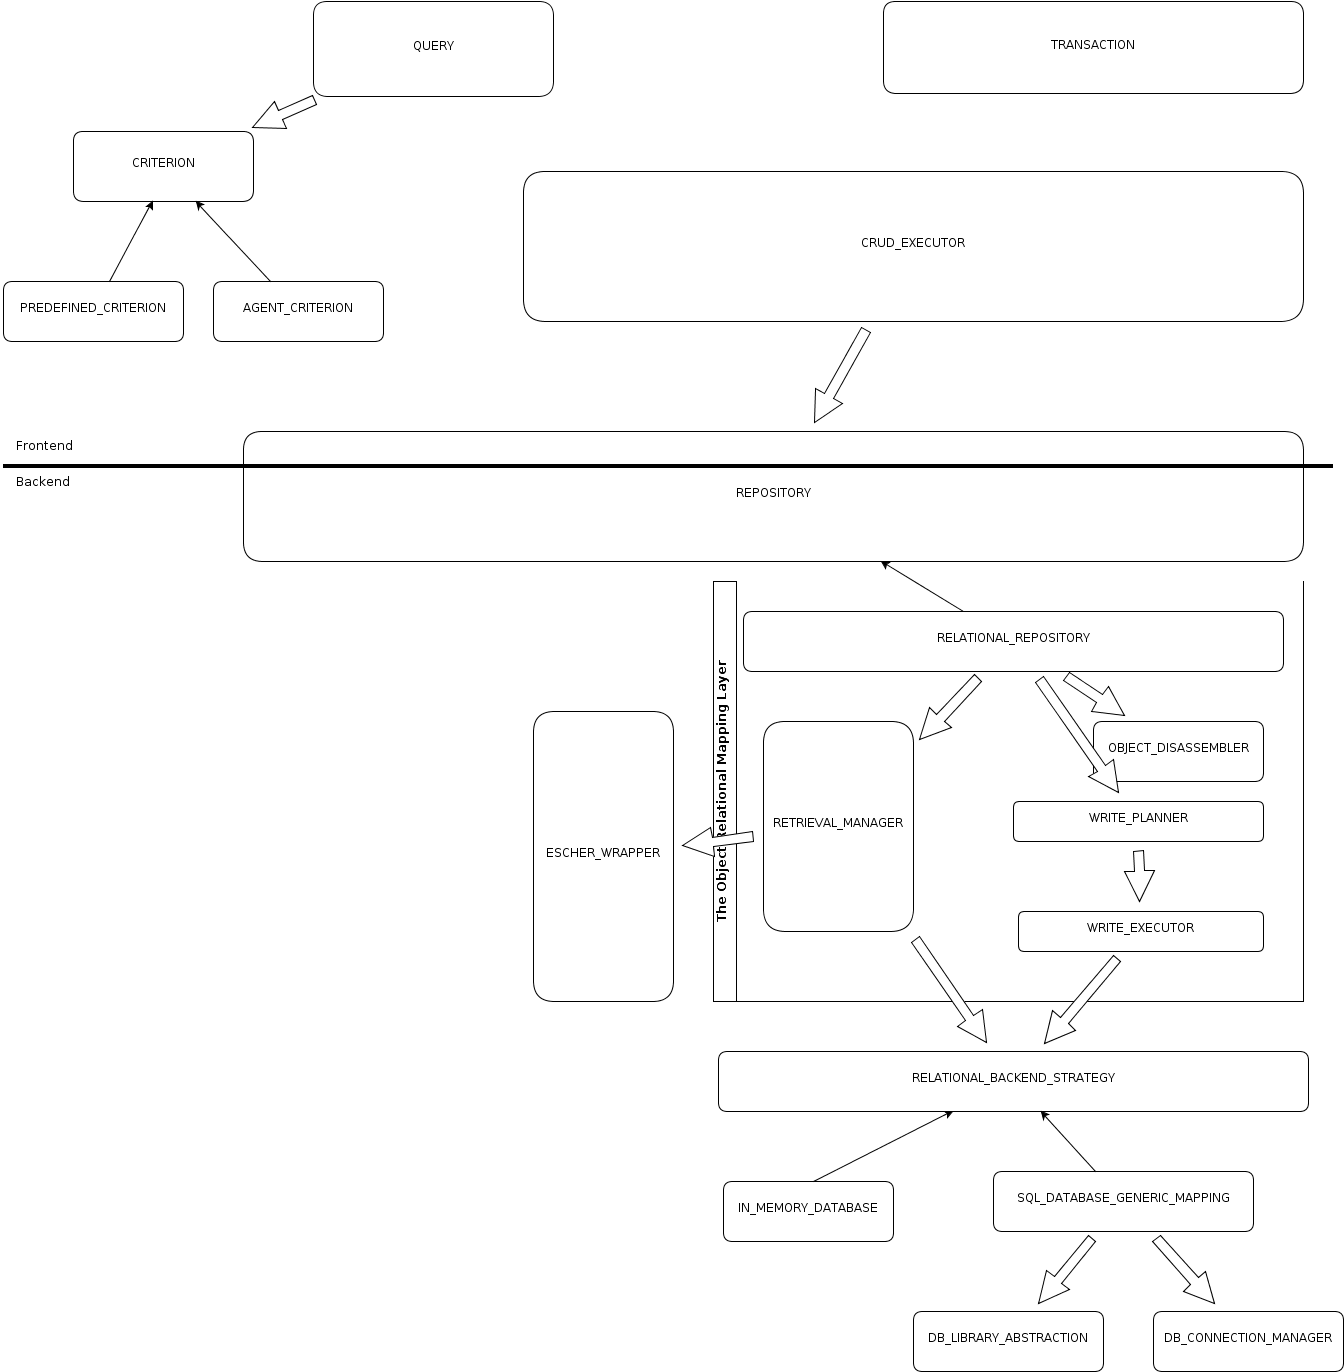
\includegraphics[width = 13cm] {class_diagram.png}

\section{Object-relational Mapping}
\label{section:ORM}

The object-relational mapping layer lies between the REPOSITORY and the BACKEND\_STRATEGY layer.
It mainly consists of four main classes doing the actual work, and a set of helper classes that represent an object graph.

The object graph representation classes are all in folder ``framework/object\_graph\_representation''. 
Although their main purpose is to represent an object graph, they are also used to describe a write operation (the BACKEND\_STRATEGY actually takes such objects as an argument)
These are the most important ones:

\begin{itemize}
 \item BASIC\_ATTRIBUTE\_PART represents an object of a basic type
 \item COLLECTION\_PART represents a collection, e.g. an instance of SPECIAL.
 \item SINGLE\_OBJECT\_PART: represets an Eiffel object that is neither a basic type nor a collection.
\end{itemize}

All these classes inherit from a deferred class OBJECT\_GRAPH\_PART. 
They have a builtin iteration cursor, and they share the concept of a dependency.

If an object graph part X is dependent on another part Y, then it means for example that Y has to be inserted first, because X needs its primary key as a foreign key in the database.

The four classes listed here are the ones that do the actual work:

\begin{itemize}
 \item The OBJECT\_DISASSEMBLER is responsible to create the explicit data structure for an object graph.
 \item The WRITE\_PLANNER is responsible to generate a total order on all write operations, taking care of the dependency relations.
 \item The RETRIEVAL\_MANAGER builds objects from the parts that it gets from the backend, and takes care that all referenced objects of a retrieved object get loaded as well.
 \item The COLLECTION\_HANDLER, or rather its descendants, add collection handling support to the basic ORM layer. 
 You need at least one handler for SPECIAL, but you can add handlers for other collection as well.
\end{itemize}

The object writing part is a bit more complex than the reading part, because of the dependency issue.


\todo{ Add a little visualization of the different parts}

\subsection{Collection handling}

You can extend the ORM algorithm to include collections. A collection is usually mapped differently from a normal object in the backend, e.g. through a M:N-relation table.
You need at least one handler for SPECIAL, because of its peculiarity that it doesn't have a fixed amount of fields.
But you can include any other collection, e.g. a LIST or an ARRAY.

There are two types of collections that you can create within a handler. 
The RELATIONAL\_COLLECTION is intended for a case when you have a typical database layout, with tables for a specific class and relations stored either with in the referenced object table (1:N-Relations) or inside their own table (M:N-Relations).
The OBJECT\_COLLECTION is intended for a scenario where you can store collections in a separate table, having their own primary key, and with the collection owner using this key as a foreign key.

Note that the choice of the collection has an effect in the object-relational mapping layer already:
\begin{itemize}
 \item An OBJECT\_COLLECTION is handled like a SINGLE\_OBJECT\_PART: The owner of the collection object depends on the collection, and the collection depends on all items that it references.
 \item A RELATIONAL\_COLLECTION in an M:N mapping mode depends on both the collection owner and all items that it references, but the owner does not depend on its collection.
 This comes from the fact that you need both a foreign key of the owner and the collection items to insert a row in a M:N-relation table
 \item A RELATIONAL\_COLLECTION in an 1:N mapping mode actually isn't forwarded to the backend at all. Instead, for each collection item there is a dependency added to the collection owner.
 Again, this comes from the normal practice in database layouts for 1:N relations.
\end{itemize}

The following diagram shows an example entity-relationship model for each type of collection:

\todo{Add model}


If you use one of the predefined backends, you usually don't have to care about collection handlers.
They become important however if you want to adapt ABEL to a custom database layout, as you can see in section ~\ref{subsection:specific_adaption}.

Please note that the framework itself does not provide any collection handler, and inserting a SPECIAL object without setting an appropriate handler will result in a runtime crash.
However, there is a SPECIAL handler shipped with the predefined backends, and e.g. the IN\_MEMORY\_REPOSITORY makes use of it.

\subsection{Object graph settings}

First, let's define the object graph more exactly, using graph theory.
A vertex in the graph corresponds to an object, and a reference is a directed edge.

The (global) object graph is the web of objects and references as it is currently in main memory.

An object Y can be ``reached'' from another object X if there is a path between X and Y, i.e. Y is in the transitive closure of X.

The object graph of an object X is an induced subgraph of the global object graph which contains all vertices that can be reached from X.

The level of an object Y in the object graph of X is the length of the shortest path from X to Y.

Using these definitions we can now describe how ABEL handles object graphs, and how you can tweak the default settings to increase performance.

Every operation in ABEL has its own depth parameter (defined in OBJECT\_GRAPH\_SETTINGS), which has the following effect:
Each operation will only handle the objects when the following condition holds: $ level(object) < depth $

Now, let's put this in a context:
You already know that the insert and retrieve features handle the complete object graph of an object. 
In fact, the depth for both functions is infinity by default.

On the other hand, the update or delete operations only handle first object they get, and don't care about the object graph.
Their depth is defined as exactly 1, which means that only an object with a level of 0 satisfies the condition above.
The only object with level 0 is in fact the root object of the object graph.

To fully understand the behaviour of ABEL, we also have to look at what happens when the algorithm reaches the ``last'' object, i.e. when the condition $level + 1 = depth$ holds.
In that case the object with all basic attributes gets inserted/updated, but references only get written if the referenced object is already persistent.
If it isn't persistent, then in a later retrieval operation the reference will be Void.

You can change the depth of the individual operations in REPOSITORY.default\_object\_graph. 
Please keep in mind that this is a dangerous operation, as a not fully retrieved or inserted object will contain Void references even in a void-safe environment, and it's also possible that they violate the invariant.

Apart from the depth, there are some other settings as well, i.e. what ABEL should do if it finds an already persistent object along the object graph of a new object to insert, or vice versa.

\section{Backend abstraction}

ABEL provides some powerful abstractions to be able to support many different storage engines. 
The three main levels of abstraction are the REPOSITORY class, the BACKEND\_STRATEGY and the database wrapper classes.

\subsection{REPOSITORY}

The deferred class REPOSITORY is the highest level of abstraction.
It deals with raw Eiffel objects and always deals with the complete object graph of such an object.
It provides a good interface for persistence mechanism that provide a similarly high level of abstraction, like for example db4o \todo{reference db4o}.

At the moment, only the RELATIONAL\_REPOSITORY implements REPOSITORY.
The RELATIONAL\_REPOSITORY uses the object-relational mapping layer and uses a generic BACKEND\_STRATEGY to perform the operations at a lower level.

\subsection{BACKEND\_STRATEGY}

The second important level of abstraction is the deferred class BACKEND\_STRATEGY.
This layer deals with one object graph part at once, either a single object or a collection.
It is responsible to map these to the actual persistence mechanism, which is usually a specific layout in a database.
Its use however is not restricted to relational databases.
The IN\_MEMORY\_DATABASE for example implements this interface to provide a fake storage engine useful for testing, and it is planned to wrap the serialization libraries using this abstraction.

\subsection{Database wrapper}


The last layer of abstraction is a set of wrappers to a database. 
It consists of three deferred classes: 
\begin{itemize}
 \item The SQL\_DATABASE\_ABSTRACTION represents a database. The main function is to acquire or release a SQL\_CONNECTION\_ABSTRACTION.
 \item The SQL\_CONNECTION\_ABSTRACTION represents a single connection. 
Its main responsibility is to forward SQL statements to the database and to represent the result in an iteration cursor of SQL\_ROW\_ABSTRACTIONs.
Another important task is to map database errors to ABEL ERROR instances.
  \item The SQL\_ROW\_ABSTRACTION represents a single row in the result of an SQL query.
\end{itemize}

The wrapper is very useful if you want to easily swap e.g. from a MySQL database to SQLite

However, keep in mind that its abstraction is not perfect. 
For example, the wrapper doesn't care about the different SQL variations, as it just forwards the statements to the database.

To overcome this problem, you can put all SQL statements in your implementation of BACKEND\_STRATEGY into a separate class and generally stick to standard SQL as much as possible.


\section{Extensions}

Due to its very flexible abstraction mechanism, you can easily extend ABEL with features like transaction management or ESCHER \todo {reference escher} integration.
The pattern how to do this is quite simple: 
You can implement a BACKEND\_STRATEGY which uses another instance of BACKEND\_STRATEGY, but does some processing on the intermediate result.
That way you can add:

\begin{itemize}
 \item Filter support for some non-persistent attributes by removing them from the OBJECT\_GRAPH\_PART during a write, and adding a default value during retrieval.
 \item ESCHER support by checking on the version attribute during a retrieval, and calling the conversion function if necessary.
 \item Client-side transaction management by using a multiversion concurrency control mechanism and delaying write operations until you can definitely commit.
 \item Caching of objects
 \item An instance that does correctness checks, e.g. by routing the calls to two different backends and comparing if the results are the same.
 \item Anything else you can imagine...
\end{itemize}

The really nice thing is that you can do that without adding complexity to the core of ABEL, and for all possible implementations of BACKEND\_STRATEGY at once.


\section{Database adaption}

The BACKEND\_STRATEGY interface allows to adapt ABEL to a lot of database layout.
Shipped with the library is a backend that uses a generic database layout which is suitable for all kinds of objects, which is explained in the next section.
But you can also adapt ABEL to your very own private database layout, as described in section ~\ref{subsection:specific_adaption}

\subsection{The generic layout backend}

The layout in the database is based upon metadata of the class. It is very flexible and allows for any type of objects to be inserted:

\todo {Add Entity-Relationship model}

In fact, this is a simplified view. 
The real model uses another relation between value and class to determine the runtime type of a value, which is required in some special cases.

The generic layout backend, located in ``backends/generic\_database\_layout'', maps Eiffel objects to this layout.

It is split into three main classes:
\begin{itemize}
 \item The METADATA\_TABLES\_MANAGER is responsible to read and write tables ``ps\_class'' and ``ps\_attribute''.
 \item The GENERIC\_LAYOUT\_SQL\_BACKEND actually implements BACKEND\_STRATEGY and is responsible to write and read the ps\_value table
 \item The GENERIC\_LAYOUT\_SQL\_STRINGS collects all SQL statements needed by the other classes. Its descendants adapt the statements to a specific database if there is an incompatibility.
\end{itemize}

The functionality of the metadata table manager is quite easy:
It just caches both metadata tables in memory and provides features to get the primary key of an attribute or a class.
If the class is not present in the database, then it will insert it and return the new primary key.

A write operation is now possible, as all required information is available: 
The attribute value in the SINGLE\_OBJECT\_PART, the attribute foreign key from the METADATA\_TABLES\_MANAGER, and the object primary key either stored in the KEY\_POID\_TABLE or generated during an insert.

The retrieval operations is similar.
You can get all attribute primary keys of a specific class from the METADATA\_TABLES\_MANAGER and then execute an SQL query which returns all values whose attribute foreign key is in the set of primary keys retrieved before, sorted by the object primary key.


\subsection{Adaption to a custom database layout}
\label{subsection:specific_adaption}

Adapting ABEL to a specific database layout needs two steps:
 \begin{itemize}
  \item Implement a BACKEND\_STRATEGY for your layout
  \item Implement COLLECTION\_HANDLERS for all collections that need to be mapped relationally
 \end{itemize}

Let's consider a very simple example. You only have two classes PERSON and ITEM:

\begin{lstlisting}[language=OOSC2Eiffel, captionpos=b, caption={Application classes}, label={lst:example_application}]
class PERSON

feature
	name:STRING

	items_owned: LINKED_LIST [ITEM]
end


class ITEM

feature
	value:INTEGER

end
\end{lstlisting}

In the database, there is table Person with columns primary\_key and name, and table Item with columns primary\_key, item, and a foreign key 'owner' to Person (as it is usual in an 1:N relation)

\todo{ER-Model}

In this setup, you only need a collection handler for LINKED\_LIST.
The collection is a RELATIONAL\_COLLECTION and it is always 1:N mapped in this simple setup.
Therefore, the implementation of your (only) collection handler is very simple:

\begin{lstlisting}[language=OOSC2Eiffel, captionpos=b, caption={The collection handler for LINKED\_LIST}, label={lst:my_linked_list_collection_handler}]
class 
	LINKED_LIST_HANDLER
inherit
	PS_COLLECTION_HANDLER [LINKED_LIST [ITEM]]
feature

	create_object_graph_part (
			obj: PS_OBJECT_IDENTIFIER_WRAPPER;
			ref_owner:PS_OBJECT_GRAPH_PART; 
			attr_name: STRING;
			mode:PS_WRITE_OPERATION)
		 : PS_RELATIONAL_COLLECTION_PART [LINKED_LIST[ITEM]]
		-- Create a new part, but don't disassemble
		do
			create Result.make (obj, ref_owner, attr_name, mode, Current)
		end

	is_in_relational_storage_mode (a_collection: PS_COLLECTION_PART[LINKED_LIST[ITEM]]):BOOLEAN = True
		-- Is `a_collection' stored in relational mode?


	is_1_to_n_mapped (a_collection:PS_COLLECTION_PART[LINKED_LIST[ITEM]]): BOOLEAN = True
		-- Is `a_collection' stored relationally in a 1:N mapping?

end
\end{lstlisting}


The implementation of BACKEND\_STRATEGY is quite straightforward as well.
You just have to distinguish between PERSON and ITEM objects and insert them in the corresponding table.

Please remember that the object-rlational mapping layer adds an attribute with name ``items\_owned'' to the ITEM object, which is the default behaviour for 1:N relations.
This especially menans that you don't need to implement the relational collection write operations.

The following code listing shows the insert feature in pseudocode:

\begin{lstlisting}[language=OOSC2Eiffel, captionpos=b, caption={The collection handler for LINKED\_LIST}, label={lst:my_backend_adaption}]
class 
	MY_SIMPLE_BACKEND
inherit
	PS_BACKEND_STRATEGY
feature

	insert (an_object:PS_SINGLE_OBJECT_PART; a_transaction:PS_TRANSACTION)
		-- Inserts the object into the database
		do
			if an_object is a PERSON object then
				database.execute_sql ("INSERT INTO person (name) VALUES " + an_object.get_value ("name"))
				key_mapper.add_entry (an_object, database.execute_sql ( "Get last autoincremented primary key of Person")
			else
				-- The ORM layer has added an attribute `items_owned' in ITEM
				foreign_key:= key_mapper.primary_key_of (an_object.get_value ("items_owned"))
				database.execute_sql ("INSERT INTO item (value, owner) VALUES " + an_object.get_value ("value") + foreign_key)
				key_mapper.add_entry (an_object, database.execute_sql ("Get last autoincremented primary key of Item")
			end
		end


	key_mapper: PS_KEY_POID_TABLE
		-- Maps object identifiers to primary keys

end
\end{lstlisting}

During a retrieval operation, you similarly have to select your values from the correct table.
Note that you need the retrieve\_relational\_collection here.


%\section{Tuning performance}

%Performance rather belongs to the future work section...


%\subsubsection{Performance remarks}

%ABEL will try to let the backend do as much of the filtering as is possible, to reduce the overhead of e.g. network communication or building unnecessary objects.
%This especially means that ABEL will compile predefined queries to SQL if you have a relational database as a backend. 
%However, if there is an agent criterion OR-ed to a predefined criterion, the test can not be made in the database because you might get false negatives.
%Therefore, to have optimal performance, you should consider the following points:

%\begin{itemize}
%\item Try not to use agent criteria if you have a relational database backend.
%\item Try not to use OR on agent criteria.
%\item Try to keep OR-ed agent criteria as deep down the tree as possible (as the above OR-node defaults to true and thus is not checked for in the backend)
%\end{itemize}


%\chapter{Conclusions}
%\chapter{Results and Conclusions}
%TODO


\section{Experimental Results}
%TODO

\section{Contribution}
The main parts of our technique were taken from the Java implementation of selective capture and replay from Joshi and Orso \cite{orso05may}, however there are some aspects that differ from their implementation and are to the best of our knowledge new:

\begin{itemize}
\item Our implementation of selective capture and replay targets Eiffel as a language.
\item We instrument applications in a way, so that the same executable can be used for both capture and replay phase. This makes it possible to replay an application immediately after it was captured, without recompiling it, which would take tens of minutes up to hours in Eiffel.
\item Our technique instruments code at the callee side, whereas Joshi and Orso instrument code at the caller side. 
\item Our instrumentation code determines whether an object is observed or unobserved dynamically, and we proposed a solution to do this check with only a small performance overhead. This enables equal instrumentation in all cases of inheritance, fully supporting dynamic binding. 
\end {itemize}

\section {Limitations}
Because of its limitations, the implementation that was made during this master thesis is to be seen as a proof of concept, only a small subset of programs can be captured and replayed. Here, we will provide a list of the known limitations:

\paragraph{Field Accesses}
The fact that there exists no automated code instrumentation for field accesses, limits the use of this implementation; however it has a weaker impact than it would have in Java, because in Eiffel, OUTREAD is the only type of field access that must be recorded in order to capture and replay an application. As a consequence of this limitation, only classes that don't read from unobserved fields can be put into the observed set.

\paragraph{Manifest Strings}
Manifest strings are directly initialized by the C code, that creates a string object and then directly writes the content of the manifest string into that object. Unlike the creation of the object, which is done using normal Eiffel routines, the initialization is directly done by the C code. This implies, that there is no instrumentation code invoked that could notice the change of the object's state. If an observed manifest string created in unobserved code and then passed to observed code, this leads to a fault during replay, because no event is generated and the initialization of the string can not be replayed. By inserting manual instrumentation using \texttt{\{SPECIAL\}.note\_direct\_manipulation}, it is possible to solve this issue. However this solution is not satisfying as manifest strings are used in many places and requiring the developer to insert manual instrumentation in each of these places is not realistic. A better solution would be to change the C macros that are used by the generated code to create manifest strings, in order to invoke the management code whenever a manifest string is instantiated.

\paragraph{Selective Exports}
In Eiffel a mechanism called \emph{selective exports} \cite{oosc2} lets classes decide, to which classes their features are exported. This feature can be seen as a generalization of Javas \emph{access level modifiers}. The problem arises whenever an observed class lets an unobserved class access a feature \identifier{f}, but prohibits the capture and replay management classes, especially class \texttt{CALLER}, from access to \identifier{f}. This leads to the situation where the event log contains an INCALL to the restricted feature, but \texttt{CALLER} is unable to call that feature during replay. A special case of selective exports are creation routines, that are often exported to \texttt{NONE} in order to restrict their usage exclusively to creation calls like \inlineeiffel{(create foo.creation\_procedure)}, which does not care about export restrictions.

The case of restricted creation procedures can be solved by treating them specially and only calling them in context of object creation. The reflection library generated by Erl-G already makes this distinction and can be used in order to replay them correctly. However, this only solves a part of the problem, all other cases of restricted access are not addressed by this solution. The only reasonable possibility to address all problems that come with selective exports, is a native reflection support in Eiffel with the option to ignore access restrictions. Native reflection support would improve the compile times of capture and replay enabled applications significantly, by not doubling the amount of classes and not making all classes part of the system. For a wider applicable implementation of selective capture and replay, native reflection support is indispensable.

\paragraph{Language Features}
At the moment only a subset of the Eiffel language features is supported. In the following we will present a list of missing features:

\begin{description}
 \item [Pre- and Postconditions] In Eiffel it is possible to add to every routine a pre- and a postcondition. The precondition, initiated by the \keyword{require} keyword, defines what the caller of the routine must ensure in order to safely call the routine. The postcondition, initiated by the \keyword{ensure} keyword, defines what the routine ensures after execution under the assumption that the precondition was met. The developer can activate the checking of these conditions, which results in a check of the precondition before and postcondition after every routine execution.\\
 Pre- and postcondition consist of a sequence of boolean Eiffel expressions, that contain function calls and attribute accesses. Thus when checking pre- and postconditions during application execution, additional events for selective capture and replay are triggered.\\
The technique must ensure that these function calls and attribute accesses do not take place during the replay phase if they are executed in the context of a unobserved routine, because it is required that unobserved code is not executed during replay phase. Furthermore it is desirable that these events are all triggered in the context of the routine the corresponding pre- and postcondition belongs to. This implies, that the instrumentation code for routine invocation must be executed before the precondition is checked and the instrumentation code for routine exit is executed after the last postcondition is checked. Otherwise the events triggered by the assertion code is executed in the context of the caller. At the moment selective capture and replay for Eiffel only works when checking of pre- and postconditions is disabled.

 \item [Class Invariants] In contrast to pre- and postcondition that express the properties of a routine, class invariants, which are initiated by the \keyword{invariant} keyword, express properties of a class. Like pre- and postconditions of routines, invariants are a sequence of boolean Eiffel expressions. They need to hold before and after all exported routines, an exception to that rule are creation procedures that establish the invariant, therefore the class invariant generally does not hold before the execution of a creation procedure.\\
The checking of the invariants can be enabled by the developer, according to the Eiffel ECMA standard \cite{Eiffel-ECMA}, they are then checked before and after every qualified routine call. As with pre- and postconditions of routines, this causes additional events during capture and replay phase, which is especially problematic for unobserved classes, which should not execute any code during replay phase. At the moment selective capture and replay for Eiffel only works with disabled invariant checking.

 \item [Exceptions] The original implementation of selective capture and replay creates an event whenever exceptions are thrown across the boundary. The current implementation for Eiffel ignores exceptions, which can cause an incorrect replay of the application, as exceptions have an impact on program flow. %Man koennte evtl. das default_rescue instrumentieren, um Exceptions einfach detektieren, allerdings muessten zusaetzlich auch alle rescue-clauses so instrumentiert werden, damit festgestellt werden kann, ob die routine eine Exception wirft --> keine einfache Sache!

 \item [Expanded Types] Variables of expanded type contain the object in contrast to regular variables that contain a reference to the object. Assigning a variable of expanded type to another variable (expanded or not) results in copying the object. Expanded types were not incorporated in the implementation of selective capture and replay for Eiffel. In general, integrating support for expanded types is no problem, but there is one thing that must be considered: it is not possible to change an expanded object in another scope than the one it is defined in, because it is not possible to reference an expanded object. Therefore it is not possible to change an expanded object originated from application code in the management code. This makes the proposed solution for OUTREAD events, modifying the target object from management code before it is accessed, inapplicable for expanded objects. One solution to this problem is to change a copy of the expanded object and assign that copy back to the original object.

 \item [Agents] Eiffel agents make it possible to wrap routines in objects. The current implementation of selective capture and replay for Eiffel has no support for agents.

 \item [Once Routines] Once routines are routines that use the \keyword{once} keyword instead of the \keyword{do} keyword. As the name suggests, once routines are executed once, at least in single threaded applications and if no special once key is defined (consult the Eiffel ECMA standard \cite{Eiffel-ECMA} for details). The current implementation does not instrument once routines, hence they are not supported. When adding support for once routines, unobserved once routines must be treated specially, because it is possible that the first call of the once routine does not come from observed code. The technique must store the result nonetheless, because it is possible that a later call will come from observed code. Therefore the first call to once function must initialize its result correctly, because any subsequent call will return the same result.
\end{description}

\paragraph{Object IDs}
In the current implementation, object IDs are not supported for instances of class \texttt{TUPLE}. This was discovered a while after they were developed and is caused by the irregular object layout that instances of class \texttt{TUPLE} have. It is possible that there are some more special cases left, although with \texttt{SPECIAL} and \texttt{TUPLE}, the usual suspects are treated.

When an object is copied using the feature \texttt{copy}, its object ID is copied, too. The correct behaviour in this case would be to request a new ID, because original and copy are two different objects and should therefore also have their own ID.

Another flaw regarding object IDs is that Eiffel's storable mechanism is not yet supported by the runtime with object ID support. Most probably this is also the reason, why Eiffel Studio using the modified runtime does not work properly.

\paragraph{Multi-Threading}
Selective capture and replay was not tested with a multi-threaded application, and some things were not designed with multi-threading in mind. One thing that certainly must be fixed in order to support multi-threading is the global counter for object IDs, which must be accessed using a mutex in order to avoid two objects, created by two threads, to have the same object ID.

When the whole management code is made thread safe, our implementation will still have the same limitation as the original one; it is required that multi-threading does not introduce any non determinism to the observed code.

\paragraph{Supported Compiler Backends}
At the moment, only frozen workbench code is supported, although most parts, like the automatically inserted instrumentation code also should work for other compiler backends, as they're implemented in pure Eiffel.


\section{Future Work}
The future work on selective capture and replay for Eiffel certainly has to focus on its current limitations. There are some limitations that restrict its usage to well prepared examples, for example the missing instrumentation of attribute accesses and the missing support for manifest strings. Making the current available features more robust is another area of work, for example the object ID support can be further improved so that they work under all circumstances. This requires additional example applications and test cases.

Native reflection support is crucial for the further success of selective capture and replay for Eiffel. The use of Erl-G is more to be seen as a workaround than a solution, because (a) there are some missing features, like access to selective exported features and (b) it raises the necessary compile time of a project enabled for selective capture and replay to hours, making it necessary to have a dedicated machine to compile the projects. No developer will accept this increase of compile time on project he is working on, therefore selective capture and replay for Eiffel is doomed in productive environments, as long as there is no native reflection support in Eiffel. But native reflection support is something that this project can not influence, this feature must be provided by the language maintainers.


\begin{flushleft}
 
{{{
\bibliographystyle {plain}
\bibliography {./references}
}}}
\end{flushleft}
\end{document}